% Asset ID: A21ParametricEquationsTikZ-001
% Source: Screenshot PDF page 1; transcript section 1; CCEA A21-CG-LO001.
% Related lesson section: Big Picture Explanation; Key Definitions and Notation.
% Purpose: Compare Cartesian and parametric representations.

\documentclass[tikz,border=8pt]{standalone}
\usepackage{amsmath}
\usepackage{pgfplots}
\pgfplotsset{compat=1.18}
\begin{document}
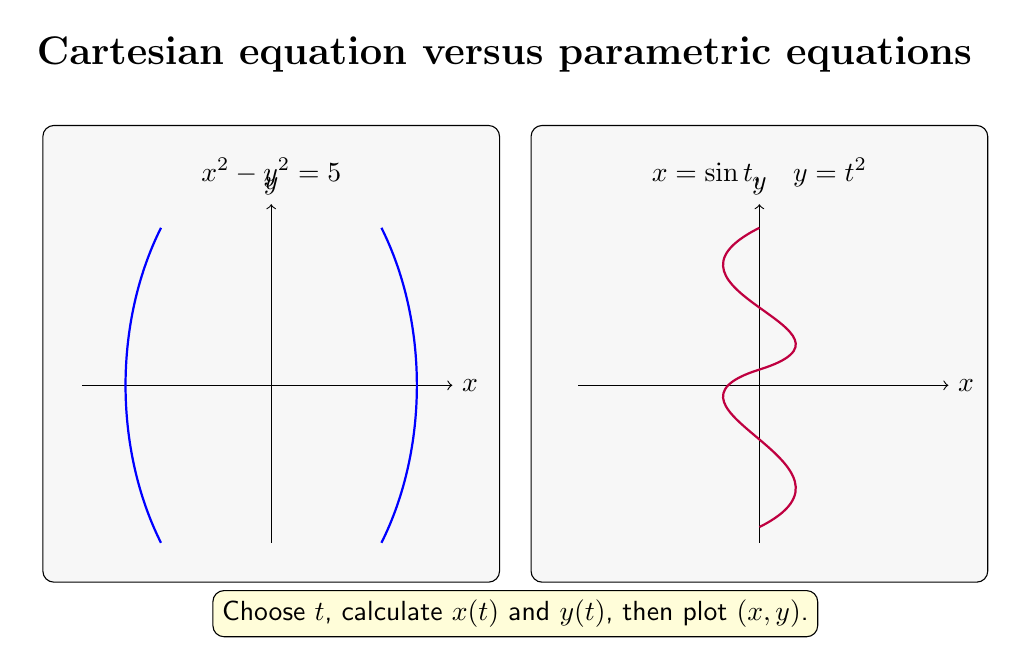
\begin{tikzpicture}[font=\sffamily]

\node[anchor=west, font=\bfseries\Large] at (-6.2,4.2) {Cartesian equation versus parametric equations};
\node[draw, rounded corners, fill=gray!6, minimum width=5.8cm, minimum height=5.8cm] at (-3.1,0.4) {};
\node at (-3.1,2.7) {\(\displaystyle x^2-y^2=5\)};
\draw[->] (-5.5,0) -- (-0.8,0) node[right] {\(x\)};
\draw[->] (-3.1,-2.0) -- (-3.1,2.3) node[above] {\(y\)};
\draw[thick, blue] (-4.5,2) .. controls (-5.1,0.8) and (-5.1,-0.8) .. (-4.5,-2);
\draw[thick, blue] (-1.7,2) .. controls (-1.1,0.8) and (-1.1,-0.8) .. (-1.7,-2);
\node[draw, rounded corners, fill=gray!6, minimum width=5.8cm, minimum height=5.8cm] at (3.1,0.4) {};
\node at (3.1,2.7) {\(\displaystyle x=\sin t,\quad y=t^2\)};
\draw[->] (0.8,0) -- (5.5,0) node[right] {\(x\)};
\draw[->] (3.1,-2.0) -- (3.1,2.3) node[above] {\(y\)};
\draw[thick, purple] (3.1,-1.8) .. controls (4.7,-1.0) and (1.5,-0.3) .. (3.1,0.2) .. controls (4.7,0.7) and (1.5,1.2) .. (3.1,2.0);
\node[draw, rounded corners, fill=yellow!15] at (0,-2.9) {Choose \(t\), calculate \(x(t)\) and \(y(t)\), then plot \((x,y)\).};

\end{tikzpicture}
\end{document}
